\documentclass[journal,12pt,twocolumn]{IEEEtran}
\usepackage{setspace}
\usepackage{gensymb}
\singlespacing
\usepackage[cmex10]{amsmath}
\usepackage{amsthm}
\usepackage{mathrsfs}
\usepackage{txfonts}
\usepackage{stfloats}
\usepackage{bm}
\usepackage{cite}
\usepackage{cases}
\usepackage{subfig}
\usepackage{longtable}
\usepackage{multirow}
\usepackage{enumitem}
\usepackage{mathtools}
\usepackage{steinmetz}
\usepackage{tikz}
\usepackage{circuitikz}
\usepackage{verbatim}
\usepackage{tfrupee}
\usepackage[breaklinks=true]{hyperref}
\usepackage{tkz-euclide}
\usetikzlibrary{calc,math}
\usepackage{listings}
    \usepackage{color}                                            %%
    \usepackage{array}                                            %%
    \usepackage{longtable}                                        %%
    \usepackage{calc}                                             %%
    \usepackage{multirow}                                         %%
    \usepackage{hhline}                                           %%
    \usepackage{ifthen}                                           %%
  %optionally (for landscape tables embedded in another document): %%
    \usepackage{lscape}     
\usepackage{multicol}
\usepackage{chngcntr}
\DeclareMathOperator*{\Res}{Res}
\renewcommand\thesection{\arabic{section}}
\renewcommand\thesubsection{\thesection.\arabic{subsection}}
\renewcommand\thesubsubsection{\thesubsection.\arabic{subsubsection}}

\renewcommand\thesectiondis{\arabic{section}}
\renewcommand\thesubsectiondis{\thesectiondis.\arabic{subsection}}
\renewcommand\thesubsubsectiondis{\thesubsectiondis.\arabic{subsubsection}}

% correct bad hyphenation here
\hyphenation{op-tical net-works semi-conduc-tor}
\def\inputGnumericTable{}                                 %%

\lstset{
frame=single, 
breaklines=true,
columns=fullflexible
}

\begin{document}


\newtheorem{theorem}{Theorem}[section]
\newtheorem{problem}{Problem}
\newtheorem{proposition}{Proposition}[section]
\newtheorem{lemma}{Lemma}[section]
\newtheorem{corollary}[theorem]{Corollary}
\newtheorem{example}{Example}[section]
\newtheorem{definition}[problem]{Definition}
\newcommand{\BEQA}{\begin{eqnarray}}
\newcommand{\EEQA}{\end{eqnarray}}
\newcommand{\define}{\stackrel{\triangle}{=}}

\bibliographystyle{IEEEtran}
\providecommand{\mbf}{\mathbf}
\providecommand{\pr}[1]{\ensuremath{\Pr\left(#1\right)}}
\providecommand{\qfunc}[1]{\ensuremath{Q\left(#1\right)}}
\providecommand{\sbrak}[1]{\ensuremath{{}\left[#1\right]}}
\providecommand{\lsbrak}[1]{\ensuremath{{}\left[#1\right.}}
\providecommand{\rsbrak}[1]{\ensuremath{{}\left.#1\right]}}
\providecommand{\brak}[1]{\ensuremath{\left(#1\right)}}
\providecommand{\lbrak}[1]{\ensuremath{\left(#1\right.}}
\providecommand{\rbrak}[1]{\ensuremath{\left.#1\right)}}
\providecommand{\cbrak}[1]{\ensuremath{\left\{#1\right\}}}
\providecommand{\lcbrak}[1]{\ensuremath{\left\{#1\right.}}
\providecommand{\rcbrak}[1]{\ensuremath{\left.#1\right\}}}
\theoremstyle{remark}
\newtheorem{rem}{Remark}
\newcommand{\sgn}{\mathop{\mathrm{sgn}}}
\providecommand{\abs}[1]{\left\vert#1\right\vert}
\providecommand{\res}[1]{\Res\displaylimits_{#1}} 
\providecommand{\norm}[1]{\left\lVert#1\right\rVert}
\providecommand{\mtx}[1]{\mathbf{#1}}
\providecommand{\mean}[1]{E\left[ #1 \right]}
\providecommand{\fourier}{\overset{\mathcal{F}}{ \rightleftharpoons}}
\providecommand{\system}{\overset{\mathcal{H}}{ \longleftrightarrow}}
\newcommand{\solution}{\noindent \textbf{Solution: }}
\newcommand{\cosec}{\,\text{cosec}\,}
\providecommand{\dec}[2]{\ensuremath{\overset{#1}{\underset{#2}{\gtrless}}}}
\newcommand{\myvec}[1]{\ensuremath{\begin{pmatrix}#1\end{pmatrix}}}
\newcommand{\mydet}[1]{\ensuremath{\begin{vmatrix}#1\end{vmatrix}}}
\numberwithin{equation}{subsection}
\makeatletter
\@addtoreset{figure}{problem}
\makeatother

\let\StandardTheFigure\thefigure
\let\vec\mathbf
\renewcommand{\thefigure}{\theproblem}



\def\putbox#1#2#3{\makebox[0in][l]{\makebox[#1][l]{}\raisebox{\baselineskip}[0in][0in]{\raisebox{#2}[0in][0in]{#3}}}}
     \def\rightbox#1{\makebox[0in][r]{#1}}
     \def\centbox#1{\makebox[0in]{#1}}
     \def\topbox#1{\raisebox{-\baselineskip}[0in][0in]{#1}}
     \def\midbox#1{\raisebox{-0.5\baselineskip}[0in][0in]{#1}}

\vspace{3cm}


\title{Assignment 1}
\author{Jaswanth Chowdary Madala}





% make the title area
\maketitle

\newpage

%\tableofcontents

\bigskip

\renewcommand{\thefigure}{\theenumi}
\renewcommand{\thetable}{\theenumi}


\begin{enumerate}
\item Find the coordinates of the focus, axis of the
parabola, the equation of the directrix and the length of the latus rectum of $y^2 = –8x$
\begin{figure}[ht]
\centering
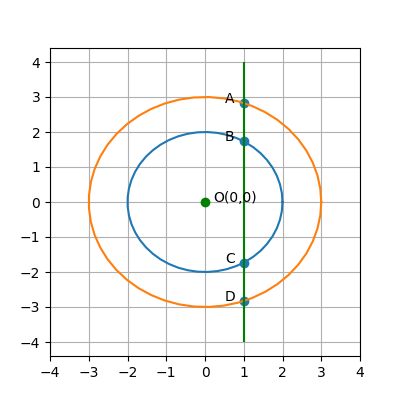
\includegraphics[width = \columnwidth]{"./figs/fig.png"}
\caption{Graph}
\label{fig:1}
\end{figure}

\textbf{Solution:}
The given equation of the parabola can be rearranged as
\begin{align}
y^2+8x = 0
\label{eq:1}
\end{align}
The above equation can be equated to the generic equation of conic sections
\begin{align}
\text{g}\brak{\vec{x}} = \vec{x}^T\vec{V}\vec{x} + 2\vec{u}^T\vec{x} + f = 0
\label{eq:2} 
\end{align}
Comparing coefficients of \eqref{eq:1} and \eqref{eq:2},
\begin{align}
\vec{V} &= \myvec{ 0 & 0 \\ 0 & 1} 
\label{eq:3}\\
\vec{u} &= \myvec{4 \\ 0} \\
f &= 0 
\end{align}

\begin{enumerate}
\item Focus: From \eqref{eq:3}, since $\vec{V}$ is already diagonalized, the Eigen values $\lambda_1$ and $\lambda_2$ are given as 
\begin{align}
\lambda_1 &= 0 \\
\lambda_2 &= 1 
\end{align}
and the eigenvector matrix
\begin{align}
\vec{P} = \vec{I}.
\end{align}

\begin{align}
\vec{p_1} &= \myvec{1 \\ 0} \\
\vec{n} &= \sqrt{\lambda_2}\vec{p_1} \\
&= \myvec{1 \\ 0} 
\end{align}

Since
\begin{align}
\label{eq:4}
c = \frac{\norm{\vec{u}^2}-\lambda_2f}{2\vec{u}^\top\vec{n}},
\end{align}
Substituting values of $\vec{u}, \vec{n}, \lambda_2 \text{ and } f$ in \eqref{eq:4}
\begin{align}
c &= \frac{4^2-1\brak{0}}{2 \myvec{4 & 0}\myvec{1 \\ 0}} = 2
\end{align}
The focus $\vec{F}$ of parabola is expressed as
\begin{align}
\vec{F} &= \frac{ce^2\vec{n}-\vec{u}}{\lambda_2} \\
&= \frac{2\brak{1}^2\myvec{1 \\0} - \myvec{4 \\ 0}}{1} \\
&= \myvec{-2 \\ 0}
\end{align}
\item Directrix: The directrix is given by
\begin{align}
\vec{n}^\top\vec{x} &= c \\
\implies	\myvec{1 & 0}\vec{x} &= 2
\end{align}

\item Axis: The equation for the axis of parabola, passing through $\vec{F}$ and orthogonal to the directrix is given as  
\begin{align}
\vec{m}^\top\brak{\vec{x}-\vec{F}} &= 0
\label{eq:5}
\end{align}
where $\vec{m}$ is the normal vector to the axis and also the slope of the directrix.
\begin{align}
\vec{n} = \myvec{1 \\ 0 }\\
\vec{m} &= \myvec{0 \\ 1} \\
\myvec{0 & 1}\myvec{\vec{x} - \myvec{-2 \\ 0}} &= 0\\
\myvec{0 & 1}\vec{x} &= 0 
\end{align}
\item Latus rectum: The latus rectum of a parabola is given by 
\begin{align}
	l &= \frac{\eta}{\lambda_2}  
	 = \frac{2\vec{u}^\top\vec{p_1}}{\lambda_2} \\
	 &= \frac{2\myvec{4 & 0}\myvec{1 \\ 0}}{1} \\
	 &= 8 \text{ units }
\end{align}
\end{enumerate}
\end{enumerate}
\end{document}